\begin{titlepage}

%\center{\fontsize{4cm}{5cm}\selectfont VOTCA-CT}
%\center{\fontsize{1.5cm}{3cm}\selectfont USER MANUAL}

\center{\huge \sc VOTCA-CTP \\ \vspace*{1cm} Charge Transport Simulations}
\vspace*{1cm}
\center{\Large \sc User Manual}

\vspace*{3cm}
\center{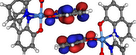
\includegraphics[width=0.6\columnwidth]{fig/logo}}
\vspace*{1cm}
\vfill

\center{\footnotesize{compiled from: \gitid}}
%\center{\footnotesize{Programs version: \refhgid}}
%\vspace*{1cm}
%\center{
%\large{\copyright \hspace*{0.1cm} VOTCA development team}
%}
\vspace*{0.5cm}
\center{\large{\today}} \\
\vspace*{0.3cm}
\htmladdnormallink{\color{black}\large{www.votca.org}}{http://www.votca.org}
\end{titlepage}

\section*{Disclamer}
Open source projects are made available and contributed to under licenses that include terms that, for the protection of contributors, make clear that the projects are offered ``as-is'', without warranty, and disclaiming liability for damages resulting from using the projects. 

\section*{Citations}
Development of this software depends on academic research grants. If you are using the package, please cite the  following papers \\

\vspace{0.1cm}
\noindent
\cite{poelking_long-range_2016} Long-range embedding of molecular ions and excitations in a polarizable molecular environment, Carl Poelking and Denis Andrienko \\
\htmladdnormallink{  {\itshape J. Chem. Theory Comp.} 12, 4516, 2016}
{http://dx.doi.org/10.1021/acs.jctc.6b00599} \\

\vspace{0.1cm}
\noindent
\cite{kordt_modeling_2016} Modeling of spatially correlated energetic disorder in organic semiconductors,
Pascal Kordt, Denis Andrienko \\
\htmladdnormallink{  {\itshape J. Chem. Theory Comput.}, 12, 36, 2016 }
{http://dx.doi.org/10.1021/acs.jctc.5b00764} \\

\vspace{0.1cm}
\noindent
\cite{ruhle_microscopic_2011} Microscopic simulations of charge transport in disordered organic semiconductors, 
Victor R\"uhle, Alexander Lukyanov, Falk May, Manuel Schrader, Thorsten Vehoff, James Kirkpatrick, Bj\"orn Baumeier and Denis Andrienko \\
\htmladdnormallink{  {\itshape J. Chem. Theor. Comp.} 7, 3335, 2011}
{http://dx.doi.org/10.1021/ct200388s} \\

\vspace{0.1cm}
\noindent
\cite{lukyanov_extracting_2010} Extracting nondispersive charge carrier mobilities of organic semiconductors from simulations of small systems, A. Lukyanov, D. Andrienko \\
\htmladdnormallink{  {\itshape Phys. Rev. B}, 82, 193202, 2010}
{http://dx.doi.org/10.1103/PhysRevB.82.193202} \\

\vspace{0.1cm}
\noindent
\cite{baumeier_density-functional_2010}
      Density-functional based determination of intermolecular charge transfer properties for large-scale morphologies, Bj{\"o}rn Baumeier,  James Kirkpatrick, and Denis Andrienko \\
       \htmladdnormallink{  {\itshape  Phys. Chem. Chem. Phys. } 12, 11103, 2010 }{http://dx.doi.org/10.1039/C002337J} \\

\vspace{0.1cm}
\noindent
\cite{ruhle_versatile_2009} Versatile Object-oriented Toolkit for Coarse-graining Applications, 
Victor R\"uhle, Christoph Junghans, Alexander Lukyanov, Kurt Kremer and Denis Andrienko \\
\htmladdnormallink{  {\itshape J. Chem. Theor. Comp.} 5, 3211, 2009}
{http://dx.doi.org/10.1021/ct900369w}

\vspace{0.1cm}
\noindent
\cite{kirkpatrick_approximate_2007} An approximate method for calculating transfer integrals based on the ZINDO Hamiltonian, James Kirkpatrick, \\
\htmladdnormallink{  {\itshape  Int. J. Quantum Chem.} 108, 51, 2007}{https://doi.org/10.1002/qua.21378}

\section*{Copyright}
\votcactp is free software. The entire package is available under the Apache License. For details, check
the LICENSE file in the source code. The \votcactp source code is available on our homepage, \htmladdnormallink{\color{black}www.votca.org}{http://www.votca.org}.

\vfill
